% Active lead circuit: the scanned schematic (active_lead.png) with the signal
% labels drawn over it in red. Build with `make figures/active_lead.pdf`.
%
% Coordinates are in the scan's own pixels, origin top left, y pointing down,
% so a label is moved by nudging the numbers.
\documentclass[border=0pt]{standalone}
\usepackage{tikz}
\usetikzlibrary{arrows.meta}

\begin{document}
\begin{tikzpicture}[x=0.01cm, y=-0.01cm,
    lbl/.style={red, font=\small},
    flow/.style={red, thick, -{Stealth[length=5pt]}}]
  % crop the cut-off "(b)" along the top of the scan
  \useasboundingbox (0,14) rectangle (678,282);
  \clip (0,14) rectangle (678,282);
  \node[anchor=north west, inner sep=0] at (0,0)
    {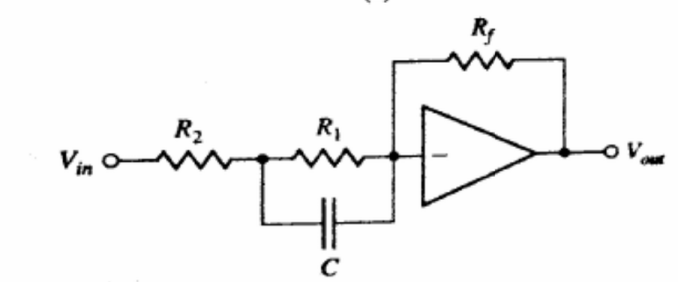
\includegraphics[width=6.78cm]{active_lead.png}};

  % currents
  \draw[flow] (123,160) -- (150,160) node[lbl, midway, above=1pt] {$i_2$};
  \draw[flow] (271,160) -- (291,160) node[lbl, midway, above=1pt] {$i_1$};
  \draw[flow] (275,222) -- (310,222) node[lbl, midway, below=1pt] {$i_c$};
  \draw[flow] (402,61)  -- (434,61)  node[lbl, midway, above=1pt] {$i_f$};

  % voltages, + on the end the current enters
  \node[lbl] at (163,187) {$+$};  \node[lbl] at (196,191) {$v_2$};  \node[lbl] at (230,187) {$-$};
  \node[lbl] at (293,187) {$+$};  \node[lbl] at (326,191) {$v_1$};  \node[lbl] at (358,187) {$-$};
  \node[lbl] at (441,88)  {$+$};  \node[lbl] at (476,92)  {$v_f$};  \node[lbl] at (511,88)  {$-$};
\end{tikzpicture}
\end{document}
